\documentclass[conference]{IEEEtran}
\IEEEoverridecommandlockouts
% The preceding line is only needed to identify funding in the first footnote. If that is unneeded, please comment it out.
\usepackage{cite}
\usepackage{amsmath,amssymb,amsfonts}
\usepackage{algorithmic}
\usepackage{graphicx}
\usepackage{textcomp}
\usepackage{xcolor}
\def\BibTeX{{\rm B\kern-.05em{\sc i\kern-.025em b}\kern-.08em
    T\kern-.1667em\lower.7ex\hbox{E}\kern-.125emX}}
    

\newcommand{\TODO}[1]{\color{green} #1 \color{black} \\}
    
\begin{document}

\title{Intelligent Systems I - Group Assignment
% {\footnotesize \textsuperscript{*}Note: Sub-titles are not captured in Xplore and
% should not be used}
% \thanks{Identify applicable funding agency here. If none, delete this.}
}

\author{\IEEEauthorblockN{1\textsuperscript{st} João Santos (76912)}
\IEEEauthorblockA{\textit{DETI} \\
\textit{Universidade de Aveiro}\\
Aveiro, Portugal \\
santos.martins.joao@ua.pt}
}

\maketitle

\begin{abstract}
In the proposed assignment it was asked for the students to build a intelligent system capable of taking thoughtful actions that, hopefully, lead an army to defend a base as long as possible. The game is composed by an allied army which the goal is to defend its base while an attacking army does what it can to destroy it. The developed agent was capable of defending the base considerably longer than the default strategy.
\end{abstract}

\begin{IEEEkeywords}
army, game, agent, intelligent systems
\end{IEEEkeywords}

\section{Introduction}


An intelligent agent is anything that observes its surroundings, acts autonomously to achieve goals, and can learn or use knowledge to enhance its performance. In the scope of this assignment, the aim was to developed such an agent that could manage resources and defend a military base by coordinating the allied soldiers against the enemy. 





The game happens in turns. In each, first the agent (or allied) moves are applied and then the enemy has its turn. If the agent takes longer than two hundred milliseconds to apply its moves, then they are ignored. Also, it can not take more than five hundred actions. If the agent can survive for two thousand turns, then it wins the game.

In this game, their are four kinds of entities:
%
\begin{enumerate}
    \item Base: this base is where the allied soldiers are recruited and the resources are obtained. It can be upgraded so, at each turn, more resources are gained;
    \item Allied Melee: these soldiers can only attack the enemy when they are on the same cell. Their elimination ratio is 1:1, this is, on melee can only attack and eliminate one enemy. Each one costs fifty resources;
    \item Allied Ranged: these soldiers can attack an enemy when it is within a three cell (Manhattan) distance. Their elimination ratio is 4:1, this is, a single ranged soldier can eliminate one enemy at three, two or one cells of distance plus another one when in the same cell. Each one costs one hundred fifty resources;
    \item Enemy Melee: these are the soldiers that will try to attack the base or any of the allied soldiers. They move towards the closest goal.
\end{enumerate}



Also, two game difficulties exist for the agents to be tested. On the easier difficulty 0, the enemies are spawn in a random position, always along the last column of the board. The base cost for upgrading the base is five hundred while the base production is two hundred.

On the harder difficulty 1, the enemies spawn on a backslash formation. The base upgrading cost eight hundred and the base production is still two hundred.

These base values are what define how much it costs to upgrade the base throughout the game and how much it will produce at each level.






\section{General Architecture}

In a macro point of view, the developed agent differentiates its behaviour (from now on called macro strategy) accordingly to the known difficulty of the game. Mainly, the agent loads a set of parameters and chooses the accordingly individual strategy (called micro strategy) for each cell with any allied soldier (melee, ranged or base). Yet, both macro strategies have big similarities.

Both macro strategies consist on building a defence block composed of ranged soldiers, while the melee soldiers try to attack the enemy by reaching the last column of the board. While this happens, the base upgrades its level in steps, this is, given a set of conditions that will be detailed in the coming sections, it stops spawning any soldier so all the generated resources are invested in the upgrading process. This conduct switches back to the default buy strategy when a desired level is reached.

A relevant part of the strategy consists in, initially, build the defense block by filling the cells with fifty ranged soldiers. When the final desired level of the base is reached, this amount switches to the maximum that is capable of the ranged attack (five hundred) which hugely increases the score reached. In the in-between a a middle amount (two hundred and fifty) is used.

\section{Main Algorithms and Parameters}

As mentioned, each difficulty caused certain specificities in the strategy.

\subsection{Difficulty 0}

Before going any further, we need to define the concept of battle front. In the scope of this project, the battle front if the farthest column that a allied ranged soldier will occupy of the battle formation. It is in this column where these soldiers will wait and attack the coming enemy. 

In the same way, the formation rows are the rows that these same ranged soldiers can occupy. Both concepts are visible on Fig. \ref{fig:dif0_formattions}. For difficult 0, the battle front was at column twenty while the formation rows where all except the middle one. When the last upgrade level is reached, the formation moves forward to column twenty five to increase the pressure in the enemy.

On the easier difficulty, the enemies spawn in random cells, i.e. they have no formation. This allows the melee soldiers to find "holes" in the attack of the enemy so that it can reach the last column of the board. To do so, the melee soldiers are always recruited on the center row (the row where the base is located) and move forward until the battle front is reached.

When the battle front is reached, three actions can happen: 
%
\begin{enumerate}
    \item if there is no enemy in the next two cells then move forward;
    \item if going forward is not a feasible solution, check if going up or down will put the melee soldiers in danger of dying in the next turn. If not, then choose one at random and move there;
    \item when all other options failed, simply move backwards in the hope than a better escape opportunity appears. If it does not, and the soldiers can not go backwards any further, sacrifice themselves for a greater good.
\end{enumerate}

Notice that all this happens for both melee soldiers that are and are not hidden. The two cell check for moving forward is needed because if less, then in a turn where both the allied and enemy move forward, they would end up in the same cell and, as a result, in an unwanted clash.

In parallel to this, the ranged soldiers are working in building the defence block. The defense block consists in moving towards the battle front and occupying all the formation rows with a given amount soldiers, as already explained. When the battle front is fully occupied, the immediately previous column is filled in the same way, and so on until the game ends or no more columns are free. When the enemy can reach and eliminate some or all the allied soldiers, then the formation is rebuilt by the soldiers on the back column moving forward.

In this difficulty, the formation rows are all except the middle one. This is intend so that the melee soldier have where to pass towards their goal. 

Given that a ranged soldier can only eliminate enemy soldiers if it is stationary, before each movement a check is performed. If an enemy is present at a distance equal or shorter than three cells (Manhattan distance) then the soldiers will not move. This happens whatever the current goal and position are. In code, this is a simple breadth-first search tree that starts with the closer cells and expands one unit distance at each time until if finds an enemy or the distance is greater than three.

Finally, the missing piece is the behaviour of the base. In the beginning, the base is upgraded whenever possible (the amount of resources is greater than the upgrade cost). When level seven is reached, the base stops the first phase of upgrading and switches to a buy strategy in order to start building some defences. The strategy consist in buying all the ranged soldiers possible with the current resources, but considering that we will want to buy, at most, twenty melee soldiers. This option was taken so that a good equilibrium between attacking and defending is gained.

Notice that, in this difficulty, it is desired to have the center row free for the melee soldiers to pass and attack the enemy. This is the reason why the melee soldiers are recruited of the cell in front of the base while the ranged are split in half and recruited in both the top and bottom cells adjacent to the base. Fig. \ref{fig:dif0_formattions} shows the general idea of the formations.

A second upgrading step for the base when the ranged soldier fully occupy the first two columns of the battle front (with 250 soldiers per cell), taking the base up to the level sixteen. The third and final step, the one that takes the base up to the final level of twenty three, happens when the same columns are again fully occupied, but with 500 soldiers per cell.

As an emergency action, if during any of the upgrading steps, the battle front soldiers happen to be attacked en eliminated, the base immediately starts recruiting more soldiers (using the same policy) until that column formation is rebuilt. 

\begin{figure*}[htbp]
    \centering
    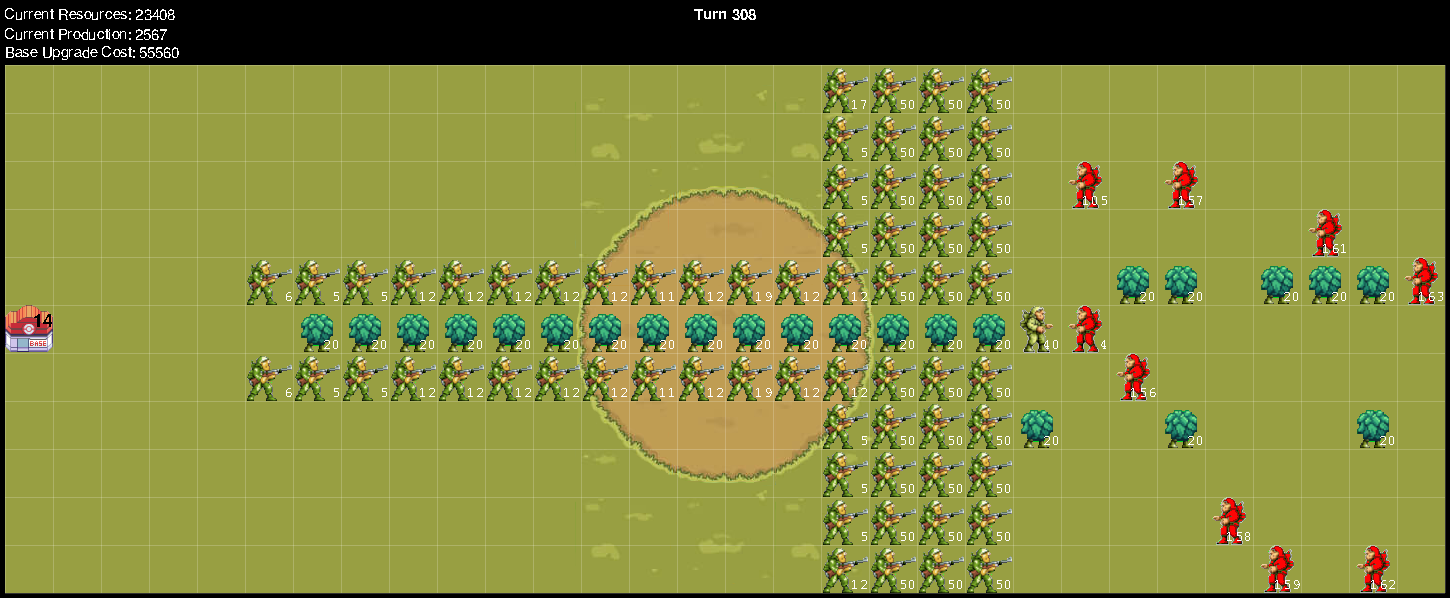
\includegraphics[width=\textwidth]{imgs/dif0_formattions.png}
    \caption{Example frame of the adopted strategy for difficulty 0.}
    \label{fig:dif0_formattions}
\end{figure*}

\subsection{Difficulty 1}

On the harder difficulty, the macro strategy is very similar, while the micro strategies differ. The first difference is that the battle front is closer to the base to give time for the ranged soldiers to gather in their positions (see Fig. \ref{fig:dif1_formattions}). Further in the game, this also changes by going forward, as in previous difficulty.

\begin{figure*}[htbp]
    \centering
    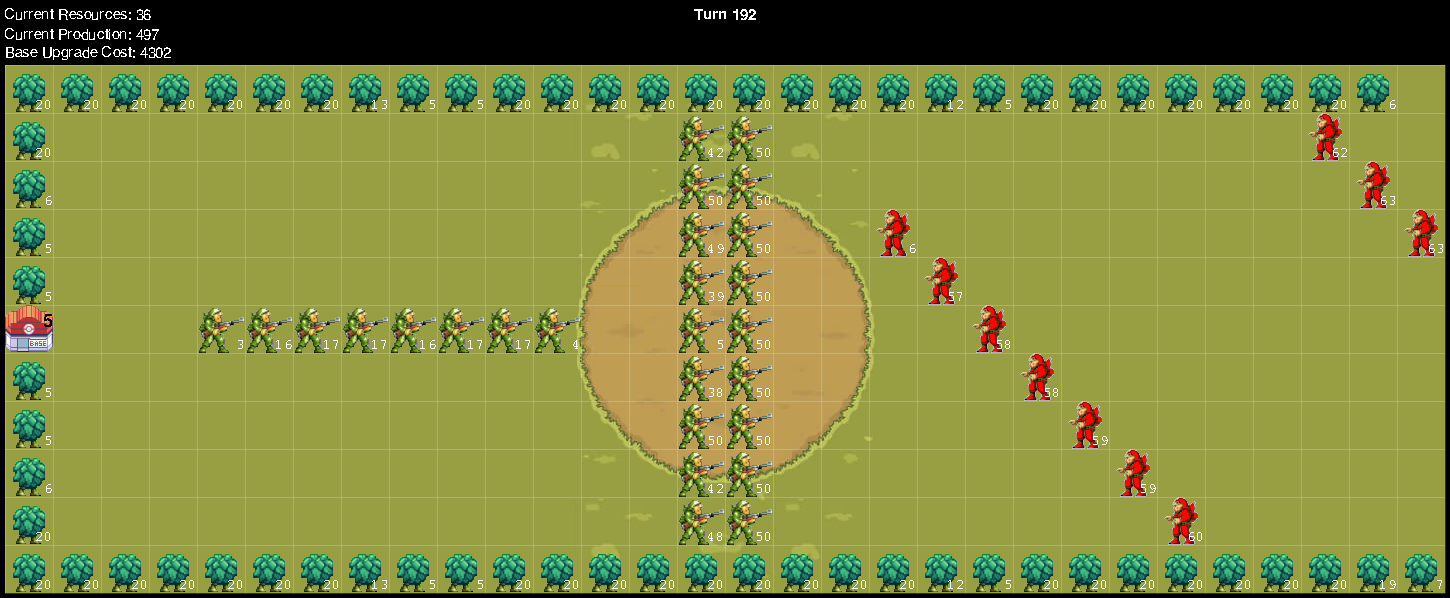
\includegraphics[width=\textwidth]{imgs/dif1_formattions.png}
    \caption{Example frame of the adopted strategy for difficulty 1.}
    \label{fig:dif1_formattions}
\end{figure*}

Also, since now the enemies appear in a diagonal formation, there are no holes that the melee soldiers can take advantage of. As a counterpart, it takes a known (and longer) number of turns for an enemy soldier to spawn in the same row. This makes it more beneficial for the melee soldiers to attack through the top and bottom rows. The formation behaviour of the enemies makes it unfeasible to try to avoid them. So, to save resources, the melee soldiers are only recruited while they (in the hidden amount) can successfully reach the last column. When the enemy spawns are so large that they can not, they stop. 

Given the increased costs on this difficulty, the author decided to maintain three steps on the upgrade strategy. Still, they happen as follows: in the start, the base is only upgraded up to level five. Then, when the first two columns on the battle front are completed with squads composed of two hundred and fifty ranged soldiers, the second step starts and goes to level sixteen. The final step takes the base to level eighteen and occurs when the those columns of the battle front are filled in the maximum amount of 500 ranged soldiers per cell.

After this point, at each turn the maximum possible amount of ranged soldiers are recruited and the agent keeps trying to hold the army positions until the enemies spawns are so large that they can punch holes on the army.

The most important parameters of this implementation have already been mentioned: battle front (column), formation rows and when the base upgrade happens and to what level. Given the define strategy, namely for difficulty 1, level eighteen is the most feasible that could be set. When trying to upgrade to any further, it would not be reached because it gives time for the enemy to start creating holes on the defense. Contrarily, on difficulty 0, going further than level twenty three provided no measurable benefit since it would take too long and too many resources to give very little reward. 

\section{Implementation Alternatives}

The initial idea to solve this assignment was to use a neural network that would learn the best strategy for the game. Unfortunately, the author did not successfully implement it. The major issue was that this should be a multi-agent neural network. The author tried to train a general neural network that would then decide the best action for each cell with a allied soldier. It was implemented by iterating over all cells with allied soldiers and then using the network to predict the best action. The network would be able to output the following set of actions:

\begin{itemize}
    \item do nothing;
    \item move all soldiers up, down, left or right;
    \item split, horizontal or vertically, the soldiers in half;
    \item upgrade the base;
    \item recruit the maximum possible amount of melee or ranged soldiers.
\end{itemize}

As outputs, it would require information about the current resources, difficulty, upgrade cost, current production, position, amount and the type and quantity of the cells within a distance of three cells.

As there was no easy or feasible way to measure how good an action is in the long term, all the network learned was to make no moves, which was not very helpful.

This lead the author to implement a more classical approach, using a a blend between a decision tree and a state machine.

\section{Performance Analysis}

As mentioned earlier, the time limit for the agent to take a set of actions was two hundred milliseconds. The implemented solution takes, in average, between ten and twenty milliseconds. This is clearly bellow the imposed limit and may suggest that a more complex agent should, maybe, be implemented to take advantage of all the time available, but only if that granted a higher score.

It is worth mentioned that this limit was not an issue during the agent development.




\section{Results}

In a five game mean, the developed agent is capable of reaching a score of 1651 at difficulty 0 and 1457 at difficulty 1. Additionally, the agent is able to inflict damage on the enemy, measured by the retard. The final (mean) scores for difficulty 0 and 1 were, respectively, 2864.2 and 3929.2.

A note should be given to the strategies of the allied melee soldiers. The author had idealized that these soldiers, in addition to their attack goal, could be used to allure the enemies in such way that would be beneficial for the defense. However, all the tested methods caused the same problem. While being allured, the enemies would gather in amount that would, in the medium term, severely harm the overall defense. This is the reason why the only goal of the melee soldiers is to stay hidden and reach the last column.

\section{Conclusion}

On the whole, the author believes that the major goals of the assignment were achieved. Not only the developed agent is able to control and take deliberate actions to protect its base, but also can intentionally attack the enemy while that is beneficial. 

Unfortunately, learning algorithms were not successfully implemented. In counterpart, this assignment actually required other concepts that were more inline with the classes.






% \section{Ease of Use}

% \subsection{Maintaining the Integrity of the Specifications}

% The IEEEtran class file is used to format your paper and style the text. All margins, 
% column widths, line spaces, and text fonts are prescribed; please do not 
% alter them. You may note peculiarities. For example, the head margin
% measures proportionately more than is customary. This measurement 
% and others are deliberate, using specifications that anticipate your paper 
% as one part of the entire proceedings, and not as an independent document. 
% Please do not revise any of the current designations.

% \section{Prepare Your Paper Before Styling}
% Before you begin to format your paper, first write and save the content as a 
% separate text file. Complete all content and organizational editing before 
% formatting. Please note sections \ref{AA}--\ref{SCM} below for more information on 
% proofreading, spelling and grammar.

% Keep your text and graphic files separate until after the text has been 
% formatted and styled. Do not number text heads---{\LaTeX} will do that 
% for you.

% \subsection{Abbreviations and Acronyms}\label{AA}
% Define abbreviations and acronyms the first time they are used in the text, 
% even after they have been defined in the abstract. Abbreviations such as 
% IEEE, SI, MKS, CGS, ac, dc, and rms do not have to be defined. Do not use 
% abbreviations in the title or heads unless they are unavoidable.

% \subsection{Units}
% \begin{itemize}
% \item Use either SI (MKS) or CGS as primary units. (SI units are encouraged.) English units may be used as secondary units (in parentheses). An exception would be the use of English units as identifiers in trade, such as ``3.5-inch disk drive''.
% \item Avoid combining SI and CGS units, such as current in amperes and magnetic field in oersteds. This often leads to confusion because equations do not balance dimensionally. If you must use mixed units, clearly state the units for each quantity that you use in an equation.
% \item Do not mix complete spellings and abbreviations of units: ``Wb/m\textsuperscript{2}'' or ``webers per square meter'', not ``webers/m\textsuperscript{2}''. Spell out units when they appear in text: ``. . . a few henries'', not ``. . . a few H''.
% \item Use a zero before decimal points: ``0.25'', not ``.25''. Use ``cm\textsuperscript{3}'', not ``cc''.)
% \end{itemize}

% \subsection{Equations}
% Number equations consecutively. To make your 
% equations more compact, you may use the solidus (~/~), the exp function, or 
% appropriate exponents. Italicize Roman symbols for quantities and variables, 
% but not Greek symbols. Use a long dash rather than a hyphen for a minus 
% sign. Punctuate equations with commas or periods when they are part of a 
% sentence, as in:
% \begin{equation}
% a+b=\gamma\label{eq}
% \end{equation}

% Be sure that the 
% symbols in your equation have been defined before or immediately following 
% the equation. Use ``\eqref{eq}'', not ``Eq.~\eqref{eq}'' or ``equation \eqref{eq}'', except at 
% the beginning of a sentence: ``Equation \eqref{eq} is . . .''

% \subsection{\LaTeX-Specific Advice}

% Please use ``soft'' (e.g., \verb|\eqref{Eq}|) cross references instead
% of ``hard'' references (e.g., \verb|(1)|). That will make it possible
% to combine sections, add equations, or change the order of figures or
% citations without having to go through the file line by line.

% Please don't use the \verb|{eqnarray}| equation environment. Use
% \verb|{align}| or \verb|{IEEEeqnarray}| instead. The \verb|{eqnarray}|
% environment leaves unsightly spaces around relation symbols.

% Please note that the \verb|{subequations}| environment in {\LaTeX}
% will increment the main equation counter even when there are no
% equation numbers displayed. If you forget that, you might write an
% article in which the equation numbers skip from (17) to (20), causing
% the copy editors to wonder if you've discovered a new method of
% counting.

% {\BibTeX} does not work by magic. It doesn't get the bibliographic
% data from thin air but from .bib files. If you use {\BibTeX} to produce a
% bibliography you must send the .bib files. 

% {\LaTeX} can't read your mind. If you assign the same label to a
% subsubsection and a table, you might find that Table I has been cross
% referenced as Table IV-B3. 

% {\LaTeX} does not have precognitive abilities. If you put a
% \verb|\label| command before the command that updates the counter it's
% supposed to be using, the label will pick up the last counter to be
% cross referenced instead. In particular, a \verb|\label| command
% should not go before the caption of a figure or a table.

% Do not use \verb|\nonumber| inside the \verb|{array}| environment. It
% will not stop equation numbers inside \verb|{array}| (there won't be
% any anyway) and it might stop a wanted equation number in the
% surrounding equation.

% \subsection{Some Common Mistakes}\label{SCM}
% \begin{itemize}
% \item The word ``data'' is plural, not singular.
% \item The subscript for the permeability of vacuum $\mu_{0}$, and other common scientific constants, is zero with subscript formatting, not a lowercase letter ``o''.
% \item In American English, commas, semicolons, periods, question and exclamation marks are located within quotation marks only when a complete thought or name is cited, such as a title or full quotation. When quotation marks are used, instead of a bold or italic typeface, to highlight a word or phrase, punctuation should appear outside of the quotation marks. A parenthetical phrase or statement at the end of a sentence is punctuated outside of the closing parenthesis (like this). (A parenthetical sentence is punctuated within the parentheses.)
% \item A graph within a graph is an ``inset'', not an ``insert''. The word alternatively is preferred to the word ``alternately'' (unless you really mean something that alternates).
% \item Do not use the word ``essentially'' to mean ``approximately'' or ``effectively''.
% \item In your paper title, if the words ``that uses'' can accurately replace the word ``using'', capitalize the ``u''; if not, keep using lower-cased.
% \item Be aware of the different meanings of the homophones ``affect'' and ``effect'', ``complement'' and ``compliment'', ``discreet'' and ``discrete'', ``principal'' and ``principle''.
% \item Do not confuse ``imply'' and ``infer''.
% \item The prefix ``non'' is not a word; it should be joined to the word it modifies, usually without a hyphen.
% \item There is no period after the ``et'' in the Latin abbreviation ``et al.''.
% \item The abbreviation ``i.e.'' means ``that is'', and the abbreviation ``e.g.'' means ``for example''.
% \end{itemize}
% An excellent style manual for science writers is \cite{b7}.

% \subsection{Authors and Affiliations}
% \textbf{The class file is designed for, but not limited to, six authors.} A 
% minimum of one author is required for all conference articles. Author names 
% should be listed starting from left to right and then moving down to the 
% next line. This is the author sequence that will be used in future citations 
% and by indexing services. Names should not be listed in columns nor group by 
% affiliation. Please keep your affiliations as succinct as possible (for 
% example, do not differentiate among departments of the same organization).

% \subsection{Identify the Headings}
% Headings, or heads, are organizational devices that guide the reader through 
% your paper. There are two types: component heads and text heads.

% Component heads identify the different components of your paper and are not 
% topically subordinate to each other. Examples include Acknowledgments and 
% References and, for these, the correct style to use is ``Heading 5''. Use 
% ``figure caption'' for your Figure captions, and ``table head'' for your 
% table title. Run-in heads, such as ``Abstract'', will require you to apply a 
% style (in this case, italic) in addition to the style provided by the drop 
% down menu to differentiate the head from the text.

% Text heads organize the topics on a relational, hierarchical basis. For 
% example, the paper title is the primary text head because all subsequent 
% material relates and elaborates on this one topic. If there are two or more 
% sub-topics, the next level head (uppercase Roman numerals) should be used 
% and, conversely, if there are not at least two sub-topics, then no subheads 
% should be introduced.

% \subsection{Figures and Tables}
% \paragraph{Positioning Figures and Tables} Place figures and tables at the top and 
% bottom of columns. Avoid placing them in the middle of columns. Large 
% figures and tables may span across both columns. Figure captions should be 
% below the figures; table heads should appear above the tables. Insert 
% figures and tables after they are cited in the text. Use the abbreviation 
% ``Fig.~\ref{fig}'', even at the beginning of a sentence.

% \begin{table}[htbp]
% \caption{Table Type Styles}
% \begin{center}
% \begin{tabular}{|c|c|c|c|}
% \hline
% \textbf{Table}&\multicolumn{3}{|c|}{\textbf{Table Column Head}} \\
% \cline{2-4} 
% \textbf{Head} & \textbf{\textit{Table column subhead}}& \textbf{\textit{Subhead}}& \textbf{\textit{Subhead}} \\
% \hline
% copy& More table copy$^{\mathrm{a}}$& &  \\
% \hline
% \multicolumn{4}{l}{$^{\mathrm{a}}$Sample of a Table footnote.}
% \end{tabular}
% \label{tab1}
% \end{center}
% \end{table}

% \begin{figure}[htbp]
% \centerline{\includegraphics{fig1.png}}
% \caption{Example of a figure caption.}
% \label{fig}
% \end{figure}

% Figure Labels: Use 8 point Times New Roman for Figure labels. Use words 
% rather than symbols or abbreviations when writing Figure axis labels to 
% avoid confusing the reader. As an example, write the quantity 
% ``Magnetization'', or ``Magnetization, M'', not just ``M''. If including 
% units in the label, present them within parentheses. Do not label axes only 
% with units. In the example, write ``Magnetization (A/m)'' or ``Magnetization 
% \{A[m(1)]\}'', not just ``A/m''. Do not label axes with a ratio of 
% quantities and units. For example, write ``Temperature (K)'', not 
% ``Temperature/K''.

% \section*{Acknowledgment}

% The preferred spelling of the word ``acknowledgment'' in America is without 
% an ``e'' after the ``g''. Avoid the stilted expression ``one of us (R. B. 
% G.) thanks $\ldots$''. Instead, try ``R. B. G. thanks$\ldots$''. Put sponsor 
% acknowledgments in the unnumbered footnote on the first page.

% \section*{References}

% Please number citations consecutively within brackets \cite{b1}. The 
% sentence punctuation follows the bracket \cite{b2}. Refer simply to the reference 
% number, as in \cite{b3}---do not use ``Ref. \cite{b3}'' or ``reference \cite{b3}'' except at 
% the beginning of a sentence: ``Reference \cite{b3} was the first $\ldots$''

% Number footnotes separately in superscripts. Place the actual footnote at 
% the bottom of the column in which it was cited. Do not put footnotes in the 
% abstract or reference list. Use letters for table footnotes.

% Unless there are six authors or more give all authors' names; do not use 
% ``et al.''. Papers that have not been published, even if they have been 
% submitted for publication, should be cited as ``unpublished'' \cite{b4}. Papers 
% that have been accepted for publication should be cited as ``in press'' \cite{b5}. 
% Capitalize only the first word in a paper title, except for proper nouns and 
% element symbols.

% For papers published in translation journals, please give the English 
% citation first, followed by the original foreign-language citation \cite{b6}.

% \begin{thebibliography}{00}
% \end{thebibliography}
% \vspace{12pt}
% \color{red}
% IEEE conference templates contain guidance text for composing and formatting conference papers. Please ensure that all template text is removed from your conference paper prior to submission to the conference. Failure to remove the template text from your paper may result in your paper not being published.

\end{document}
